\documentclass[12pt]{beamer}
%\documentclass[xcolor=dvipsnames]{beamer}
\usepackage[spanish]{babel}
\usepackage[utf8]{inputenc}
\usepackage{graphicx}
\usepackage[style=long,nonumberlist,toc,xindy,acronym,nomain]{glossaries}
\usepackage{natbib}
\usepackage{algorithm,algorithmic}
\usepackage{multicol}
\usepackage[dvips]{epsfig}
\usepackage{alltt}
\usepackage{multirow}
\usepackage{caption}
\usepackage{amsmath}
\usepackage{booktabs}
\usepackage{capt-of}% or use the larger `caption` package
\setcounter{MaxMatrixCols}{20}
\usepackage{amstext} % for \text macro
\usepackage{array}   % for \newcolumntype macro
\newcolumntype{L}{>{$}l<{$}} % math-mode version of "l" column type
\newcommand\Fontvi{\fontsize{10}{7.2}\selectfont}
\newcommand\Fontvii{\fontsize{8}{7.2}\selectfont}



\bibliographystyle{apalike}
% make bibliography entries smaller
\renewcommand\bibfont{\scriptsize}
% If you have more than one page of references, you want to tell beamer
% to put the continuation section label from the second slide onwards
\setbeamertemplate{frametitle continuation}[from second]
% Now get rid of all the colours
\setbeamercolor*{bibliography entry title}{fg=black}
\setbeamercolor*{bibliography entry author}{fg=black}
\setbeamercolor*{bibliography entry location}{fg=black}
\setbeamercolor*{bibliography entry note}{fg=black}
% and kill the abominable icon
\setbeamertemplate{bibliography item}{}
\newcommand{\beamer}{\textsc{beamer}}
\newtheorem{definicion}{Definición}
\newtheorem{ejemplo}{Ejemplo}

\makeglossaries
\newacronym{obl-cpso}{OBL-CPSO}{Opposition-Based Learning Competitive Particle Swarm Optimization}
\newacronym{cma-es}{CMA-ES}{Covariance Matrix Adaptation Evolutionary Strategy}
\newacronym{hsags}{HSAGS}{Hybrid Simulated Annealing with Global Search}
\newacronym{genopt}{GenOpt}{Generalization-Based Contest in Global Optimization}
\newacronym{cec}{CEC}{Congress on Evolutionary Computation}
\newacronym{gecco}{GECCO}{Genetic and Evolutionary Computation Conference}
\newacronym{gtoc}{GTOC}{Global Trajectory Optimisation Competition}
\newacronym{gs}{GS}{Global Search}
\newacronym{obl}{OBL}{Opposition-Based Learning}
\newacronym{qobl}{QOBL}{Quasi-opposition-based Learning}
\newacronym{qrobl}{QROBL}{Quasi-reflected Opposition-based Learning}

%%%%%%%%%%%%%%%%%%%%%%%%%%%%%%%%%%%%%%%%%%%%%%%%%%%%%%%%%%%%%%%%%%%%%%%%%%%%%%%
\title[Desarrollo de Algoritmos Dirigido por Retos]{Desarrollo de Algoritmos Dirigido por Retos}
\author[Alejandro Marrero Díaz]{\Huge{Alejandro Marrero Díaz}}
\institute[ULL]{Universidad de La Laguna}
\date[]{\today}
%%%%%%%%%%%%%%%%%%%%%%%%%%%%%%%%%%%%%%%%%%%%%%%%%%%%%%%%%%%%%%%%%%%%%%%%%%%%%%%

\usetheme{Madrid}

%%%%%%%%%%%%%%%%%%%%%%%%%%%%%%%%%%%%%%%%%%%%%%%%%%%%%%%%%%%%%%%%%%%%%%%%%%%%%%%
\definecolor{pantone254}{RGB}{122,59,122}
\definecolor{pantone3015}{RGB}{0,88,147}
\definecolor{pantone432}{RGB}{56,61,66}
\setbeamercolor*{palette primary}{use=structure,fg=white,bg=pantone254}
\setbeamercolor*{palette secondary}{use=structure,fg=white,bg=pantone3015}
\setbeamercolor*{palette tertiary}{use=structure,fg=white,bg=pantone432}
\setbeamercolor*{palette sidebar primary}{use=structure,fg=pantone254}
\setbeamercolor*{palette sidebar tertiary}{use=structure,fg=pantone3015}
\setbeamercolor*{block title}{bg=pantone3015,fg=white}
\setbeamercolor*{alerted text}{fg=pantone432}
\setbeamercolor*{item projected}{fg=pantone254}
\setbeamercolor*{section in toc shaded}{use=structure,fg=structure.fg}
\setbeamercolor*{section in toc}{fg=pantone3015}
\setbeamercolor*{subsection in toc shaded}{fg=pantone3015}
\setbeamercolor*{subsection in toc}{fg=pantone432}

%%%%%%%%%%%%%%%%%%%%%%%%%%%%%%%%%%%%%%%%%%%%%%%%%%%%%%%%%%%%%%%%%%%%%%%%%%%%%%%
\begin{document}
  
%++++++++++++++++++++++++++++++++++++++++++++++++++++++++++++++++++++++++++++++  
\begin{frame}
  \centering
  
\includegraphics[width=0.15\textwidth]{img/ullesc.eps}
  \titlepage

  \begin{scriptsize}
    \begin{center}
     Escuela Superior de Ingeniería y Tecnología \\
     Universidad de La Laguna
    \end{center}
  \end{scriptsize}

\end{frame}
%++++++++++++++++++++++++++++++++++++++++++++++++++++++++++++++++++++++++++++++  

%++++++++++++++++++++++++++++++++++++++++++++++++++++++++++++++++++++++++++++++  
\begin{frame}
  \frametitle{Índice}  
  \tableofcontents
\end{frame}
%++++++++++++++++++++++++++++++++++++++++++++++++++++++++++++++++++++++++++++++ 
\Fontvi

\section{Introducción}
\begin{frame}
\frametitle{Introducción}
\begin{block}{Motivación y Objetivos}
\begin{itemize}
	\item Iniciación en el mundo de la investigación.
	\item Investigación en el campo de las meta-heuristicas.
	\item Optimización Global Continua.
  \item Guiar el desarrollo de todo el TFG a través de la participación en una competición de optimización global continua.
\end{itemize}
\end{block}
\begin{block}{Competiciones}
  \begin{itemize}
  \Fontvi
  \item\gls{cec}
  \item\gls{gecco}
  \item\gls{gtoc} 
  \item\textbf{\gls{genopt}}
  \end{itemize}
\end{block}
\end{frame}



\section{Conceptos Previos}

\begin{frame}
  \centering
  
\includegraphics[width=0.15\textwidth]{img/ullesc.eps}
  \begin{scriptsize}
    \begin{center}
    \Huge{Conceptos Previos}
    \end{center}
  \end{scriptsize}
\end{frame}
\begin{frame}
    \frametitle{Optimización Global}
    \begin{block}{Definición Formal}
    El objetivo de la optimización global, considerando un problema de minimización, es encontrar un vector $X* \in \Omega$ tal que $f(X*) \leq f(X)$ para todo $X \in \Omega$.
    \end{block}
    \begin{block}{Espacio de Búsqueda}
    \textbf{El espacio de búsqueda} $\Omega$ está definido por un límite inferior ($a_{i}$) y superior ($b_{i}$) para cada una de las variables de decisión de la función, es decir: $\Omega = \prod^{D}_{i=1}[a_{i}, b{i}]$, siendo D el número de variables de decisión del problema a optimizar \citep{Segredo2017}
    \end{block}
\end{frame}

%++++++++++++++++++++++++++++++++++++++++++++++++++++++++++++++++++++++++++++++
\begin{frame} %TODO
\frametitle{Meta-heuristicas}
\begin{figure}
  \centering
	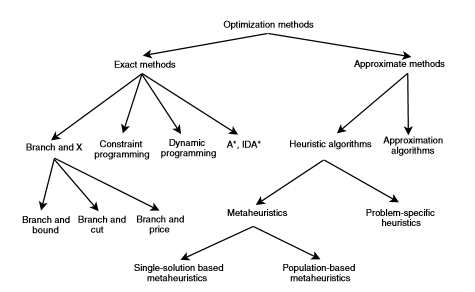
\includegraphics[scale=0.25]{img/meta}
\end{figure}
\end{frame}

%++++++++++++++++++++++++++++++++++++++++++++++++++++++++++++++++++++++++++++++
\begin{frame}
\frametitle{Meta-heuristicas}
\begin{block}{Categorías}
\begin{itemize}
    \item \textbf{Búsquedas Locales}: Greedy Randomized Adaptive Search Procedure (GRASP) \cite{GRASP}, Variable Neighborhood Search (VNS) \cite{vns}.
    \item \textbf{Heurísticas Voraces}: Simulated Annealing (SA) \cite{SA}.
    \item \textbf{Algoritmos Evolutivos}: Covariance Matrix Adaptation Evolutionary Strategy (CMA-ES) \cite{CMA}, Differential Evolution (DE) \cite{DE1, DE2, DE3}, Coevolutionary Algorithms (CEA) \cite{COE1, COE2, COE3}.
\end{itemize}
\end{block}
\end{frame}

%++++++++++++++++++++++++++++++++++++++++++++++++++++++++++++++++++++++++++++++
\begin{frame}
\frametitle{Meta-heuristicas}
\begin{block}{Criterios de Diseño}
\Fontvi
\begin{itemize}
	\item Representación.
    \begin{itemize}
    \item Permutaciones.
    \item Cadena binaria.
    \item Vector de valores naturales.
    \item \textbf{Vector de números reales}.
\end{itemize}
	\item Condición de parada.
    \begin{itemize}
    \item Iteraciones.
    \item Factor de error.
    \item \textbf{Evaluaciones}: $10^{6}$ evaluaciones establecidas por GenOpt.
\end{itemize}
	\end{itemize}
    \end{block}
\end{frame}



\begin{frame}

\frametitle{Algoritmos Desarrollados}
\begin{block}{}
\begin{itemize}
	\item\gls{obl}
	\item\gls{gs}
\end{itemize}
\end{block}

\begin{block}{}
\begin{itemize}
	\Fontvii
	\item\gls{obl-cpso}
	\Fontvi
	\item\gls{cma-es}
	\Fontvi
	\item\gls{hsags}
	\end{itemize}
\end{block}

\end{frame}

%++++++++++++++++++++++++++++++++++++++++++++++++++++++++++++++++++++++++++++++
\begin{frame}
\frametitle{Opposition-Based Learning}
\begin{block}{}
Opposition-Based Learning es un concepto en computación que ha demostrado gran efectividad a la hora de mejorar diversas técnicas de optimización.
\end{block}
\begin{block}{}
Al evaluar una solución candidata $X$ perteneciente al conjunto $S$, simultáneamente calcularemos y evaluaremos la solución opuesta $\overline{X}$.
\end{block}
\begin{block}{Variantes \cite{Segredo2017}}
\begin{itemize}
	\item\gls{qobl}
	\item\gls{qrobl}
	\end{itemize}
\end{block}
\end{frame}

\begin{frame}
\frametitle{Opposition-Based Learning}
\begin{block}{Definición formal}
Sea $x \in \Re $  un número real definido dentro de un cierto intervalo: $x \in [a,b]$. El número opuesto de x denotado como $\overline{x}$ se define de la siguiente forma \cite{obl}:
 \begin{equation}
     \overline{x} = a + b - x 
 \end{equation}
 \end{block}
 \begin{block}{Función D-Dimensional}
Sea $ P(x_{1}, x_{2},...,x_{D}) $ un punto dentro de un sistema de coordenadas $D-dimensional$ con $ x_{1},...,x_{D} \in \Re$ y además $ x_{i} \in [a_{i}, b{i}]$ \cite{obl}. El opuesto del punto P se define como las coordenadas $\overline{x_{1}},...\overline{x_{D}}$ donde:
\begin{equation}
    \overline{x_{i}} = a_{i} + b_{i} - x_{i} \quad i = 1,...,D 
\end{equation}
 \end{block}
\end{frame}

%+++++++++++++++++++++++++++++++++++++++++++++++++++++++++++++++++++++++++++++
\begin{frame}
\frametitle{Búsqueda Global}
\begin{block}{}
En ciencias de la computación, una búsqueda global (Global Search) es un método heurístico para resolver problemas complejos de optimización \cite{GlobalSearch, GlobalSearch2, GlobalSearch3}.
 \end{block}
\begin{block}{}
\begin{itemize}
	\item Explorar nuevas regiones del espacio de búsqueda $\Omega$.
	\item Equilibrio entre intensificación y diversificación.
\end{itemize}
 \end{block}
\end{frame}

\begin{frame}
\frametitle{Búsqueda Global}
\begin{block}{Centroide}
El centroide de un conjunto de $k$ elementos, tal que $k = \left | S \right |$, se define como:
\begin{equation}
    C = \frac{x_{1} + x_{2} + ... + x_{k}}{k}
\end{equation}
 \end{block}
\begin{block}{}
Cada elemento $x_{i}$ representa una solución factible a nuestro problema con $D$ variables.
 \end{block}
\end{frame}

\begin{frame}
\frametitle{Búsqueda Global}
\begin{algorithm}[H]
  \caption{Cálculo del centroide}
  \label{pseu:centroide}
  \begin{algorithmic}[1]
    \FOR{$i \leftarrow 0 $ hasta $D$}
      \STATE $Suma = 0$;
      \FOR{$j \leftarrow 0$ hasta $\left | S \right |$}
        \STATE $Suma = Suma + S[i][j];$
      \ENDFOR
      \STATE Centroide[i] = $\frac{Suma}{\left | S \right |}$;
    \ENDFOR    
    \RETURN Centroide
  \end{algorithmic}
\end{algorithm}
\end{frame}

\begin{frame}
\centering
\frametitle{Búsqueda Global}
  \scalebox{0.6}{%
  \begin{minipage}[b]{1.2\linewidth}
  \begin{algorithm}[H]
  \caption{Búsqueda global(\mbox{})}
  \label{pseu:bg}
  \begin{multicols}{2}
  \begin{algorithmic}[1]
    \STATE NumIndividuos = $\left | S \right |$;
    \STATE OrdenarPoblacion(S);
    \STATE MarcarNoExplorados(S);
    \STATE Centroide = CalcularCentroide();
    \STATE NumeroMejora = 0;
    \STATE NumeroExplorado = 0;
    \WHILE{$NumeroMejora > 0 $ y $NumeroExplorado < \left | S \right |$}
      \STATE k = 0;
      \WHILE{$S[k] = explorado $ y $NumeroExplorado < \left | S \right |$}
        \STATE k = rand(0, $\left | S \right |$); (1)
      \ENDWHILE
      \STATE S[k] = explorado;
      \STATE NumeroExplorado = NumeroExplorado + 1;
      \STATE Mejora = true;
      \WHILE{$Mejora = true$}
        \WHILE{$|a_{1}| + |a_{2}| + |a_{3}| \neq 1$}
          \STATE GenerarRand(a1, a2, a3); (2)
        \ENDWHILE
        \WHILE{$ r_{1} < k$}
          \STATE $ r_{1}$ = rand(0, $\left | S \right |$); (2)
        \ENDWHILE
        \STATE NuevoInd = ModificarIndividuo(k, a1, a2, a3, Centroide, $r_{1}$);
        \IF{$NuevoInd < S[k]$}
          \STATE $Mejora = true;$
          \STATE $S = S \cap NuevoInd$;
          \STATE NumeroMejora = NumeroMejora + 1;
          \ELSE
            \STATE Mejora = false;
        \ENDIF
      \ENDWHILE
    \ENDWHILE
    \STATE OrdenarPoblacion(S); 
    \STATE S = ObtenerMejores(0, NumIndividuos, S);
    \RETURN $\left | S \right |$ mejores individuos encontrados
  \end{algorithmic}
  \end{multicols}
\end{algorithm}
\end{minipage}}
\end{frame}


%+++++++++++++++++++++++++++++++++++++++++++++++++++++++++++++++++++++++++++++

\begin{frame}{\resizebox{\textwidth}{!}{OBL Competitive Particle Swarm Optimization (OBL-CPSO)}}
\begin{block}{Particle Swarm Optimization}
Particle Swarm Optimization (PSO) \cite{metabook, comparison, PSO_KA, GPSO} es una estrategia de optimización que ha demostrado ser muy eficiente en problemas de optimización global continua.
 \end{block}
\begin{block}{Características}
\begin{itemize}
	\item Conjunto de soluciones $S$ como un enjambre de partículas.
	\item Las partículas se mueven dentro de $\Omega$.
	\item Cada partícula posee una posición $x_{i}$ y una velocidad $\overrightarrow{v}$.
	\item Recuerdan su mejor posición alcanzada $pb_{i}$ \cite{metabook}.
	\item Mejor partícula global $gb$.
\end{itemize}
 \end{block}
\end{frame}

\begin{frame}{OBL-CPSO}
\centering
  \scalebox{0.8}{%
  \begin{minipage}[b]{1.2\linewidth}
  \begin{algorithm}[H]
  \caption{Particle Swarm Optimization(\mbox{})}
  \label{pseu:pso}
  \begin{algorithmic}[1]
    \WHILE{Condición de parada no satisfecha}
      \FORALL{$p_{i}$ en S}
        \STATE Evaluar $ p_{i} $;
        \STATE Actualizar mejor posición $pb_{i}$;
        \STATE Actualizar mejor global $gb$;
      \ENDFOR
      \FORALL{$p_{i}$ en S}
       \FORALL{$d_{i}$ en D}
       \STATE $ v_{i,d} = v_{i,d} + C_{1} * Rnd(0,1) * [pb_{i,d} - x_{i,d}] + C_{2} + Rnd(0,1) * [gb_{d} - x_{i,d}] $;\\ Rnd(0,1) devuelve un número generado aleatoriamente en el rango [0, 1]
            $ x_{i,d} = x_{i,d} + v_{i,d}$; \\
       \ENDFOR
      \ENDFOR
    \ENDWHILE
    \RETURN Mejor solución obtenida
  \end{algorithmic}
\end{algorithm}
\end{minipage}}
\end{frame}


\begin{frame}{OBL-CPSO}
\begin{block}{}
El algoritmo Opposition-based Learning Competitive Particle Swarm Optimization (OBL-CPSO) \cite{oblcpso} incluye dos modificaciones:
\begin{itemize}
	\item Opposition-based Learning.
	\item Procedimiento de Competición.
\end{itemize}
\end{block}

\begin{block}{Competición}
Escogemos, aleatoriamente, tres partículas dentro del enjambre y las hacemos competir entre ellas mediante su valor de función objetivo. 
\end{block}
\begin{block}{}
Para un enjambre de tamaño $N$, se realizarán un total de $N/3$ competiciones \cite{oblcpso}.
\end{block}
\end{frame}

\begin{frame}
\frametitle{OBL-CPSO}
\begin{block}{}
\begin{itemize}
	\item Ganadora - Winner (w): pasa directamente a la siguiente iteración.
	\item Neutra (n): utilizamos OBL.
	\item Perdedora - Loser (l): aprende de la partícula ganadora.
\end{itemize}
\end{block}
\end{frame}

\begin{frame}[shrink=20]
\frametitle{OBL-CPSO}
\begin{block}{}
\begin{equation}\label{eq:7}
    V^{k}_{ld}(t+1) = R^{k}_{1d}(t) * V^{k}_{ld}(t) + R^{k}_{2d}(t) * (X^{k}_{wd}(t) - X^{k}_{ld}(t)) + \varphi * R^{k}_{3d}(t) * (\overline{X}^{k}_{ld}(t+1)) 
\end{equation}

\begin{equation}\label{eq:8}
     X^{k}_{ld}(t+1) = X^{k}_{ld}(t) + V^{k}_{ld}(t+1)
\end{equation}

\begin{equation}\label{eq:9}
     X^{k}_{nd}(t+1) = ub_{d} + lb_{d} - X^{k}_{nd}(t) + R^{k}_{4d}(t) * X^{k}_{nd}(t)
\end{equation}

\end{block}
\begin{block}{}
Donde $X^{k}_{wd}(t)$, $ X^{k}_{ld}(t)$ y $ X^{k}_{nd}(t)$ son las posiciones d-ésimas de las w, l y n en la k-ésima ronda de competición dentro de la iteración t. \\
$V^{k}_{ld}$ es la velocidad de la partícula l en la dimensión d-ésima en la k-ésima ronda de competición de la iteración t \cite{oblcpso}. \\
$R^{k}_{1d}$, $R^{k}_{2d}(t)$, $R^{k}_{3d}(t)$ y $R^{k}_{4d}(t) \in [0, 1]$ \\
$\varphi$ es un parámetro fijado manualmente. \\
$\overline{X}^{k}_{ld}(t)$ representa el valor medio de las posiciones de las partículas dentro del enjambre. \\
$ub_{d}$ y $lb_{d}$ son las cotas superiores e inferiores del espacio de búsqueda en la dimensión d-ésima \cite{oblcpso}. \\
\end{block}
\end{frame}

\begin{frame}
\frametitle{OBL-CPSO}
\begin{block}{Problemas en la actualización}
Si una variable $x_{i}$ toma un valor fuera del rango $[a,b]: $
\begin{itemize}
    \item \textbf{$X_{id} > b$}: $X_{id} = b$.
    \item \textbf{$X_{id} < a$}: $X_{id} = a$.
    \end{itemize}
\end{block}
\end{frame}

\begin{frame}
\frametitle{OBL-CPSO}
\centering
  \scalebox{0.8}{%
  \begin{minipage}[b]{1.2\linewidth}
  \begin{algorithm}[H]
  \caption{OBL Competitive Particle Swarm Optimization(\mbox{})}
  \label{pseu:oblcpso}
  \begin{algorithmic}[1]
    \STATE Inicializar();
    \WHILE{Condición de parada no satisfecha}
      \FORALL{$ k=1: N/3 $}
        \STATE $ r_{1} = S(k)$;
        \STATE $ r_{2} = S(k + N/3)$;
        \STATE $ r_{3} = S(k + 2N/3)$;
        \STATE $(w, n, l) = competir(r_{1}, r_{2}, r_{3})$;
        \STATE Actualizar $ X^{k}_{ld}(t)$; (Ec. \ref{eq:7} y Ec. \ref{eq:8})
        \STATE Actualizar $ X^{k}_{nd}(t)$; (Ec. \ref{eq:9})
        \STATE Actualizar los valores de fitness para N y L;
      \ENDFOR
      \STATE BusquedaGlobal(); secc. \ref{sec:BG}
    \ENDWHILE
    \RETURN Mejor solución obtenida
  \end{algorithmic}
\end{algorithm}
\end{minipage}}
\end{frame}


%++++++++++++++++++++++++++++++++++++++++++++++++++++++++++++++++++++++++++++++

\begin{frame}{\resizebox{\textwidth}{!}{Covariance Matrix Adaptation Evolutionary Strategy (CMA-ES)}}
\begin{block}{}
Covariance Matrix Adaptation Evolutionary Strategy (CMA-ES) \cite{CMA1, CMA2, CMA} es un algoritmo evolutivo diseñado para problemas de optimización continua no lineales.
 \end{block}
 \begin{block}{Características}
 \begin{itemize}
 	\item Muestreo mediante Distribución Normal Multivariante.
 	\item No es necesario un gran estudio de los parámetros.
 	\item Gran abánico de posibilidades en el diseño. Reinicios y criterios de finalización.
 \end{itemize}
 \end{block}
\end{frame}

\section{Evaluación Experimental}
\subsection{Funciones Propuestas por GenOpt}
\begin{frame}
\frametitle{Funciones propuestas por GenOpt}
\begin{block}{Caracteristicas}
\textit{GenOpt} ha propuesto un total de \textbf{18 funciones} de dimensiones $D = 10, 30$ a optimizar, realizando \textbf{cien ejecuciones independientes} para cada una de ellas.
\end{block}
\begin{block}{Familias de Funciones}
\begin{itemize}
	\item Funciones GKLS.
	\item Funciones Clásicas Transformadas.
	 \begin{itemize}
    	\item Rastrigin. 
    	\item Rosenbrock. 
    	\item Zakharov. 
    \end{itemize}
	\item Funciones Compuestas.
	 \begin{itemize}
    	  	\item Goldstein-Price.
    	  	\item Hartmann. 
    	  	\item Sphere.
    	  \end{itemize}
\end{itemize}
\end{block}
\end{frame}

%++++++++++++++++++++++++++++++++++++++++++++++++++++++++++++++++++++++++++++++
\subsection{Estudio de la Parametrización y Rendimiento}

\begin{frame}
\frametitle{Estudio de la Parametrización}
\begin{block}{Objetivos del Estudio}
Determinar los mejores valores para los parámetros de cada algoritmo buscando obtener el máximo rendimiento de cada uno de ellos.
\end{block}
\begin{block}{Poblaciones}
\begin{itemize}
	\item $popsize = 20, 50, 75, 100$ para OBL-CPSO y CMA-ES.
	\item $popsize = 1$ para HSAGS.
	\end{itemize}
\end{block}
\end{frame}

\begin{frame}
\frametitle{Rendimiento de OBL-CPSO}
\begin{figure}
  \centering
	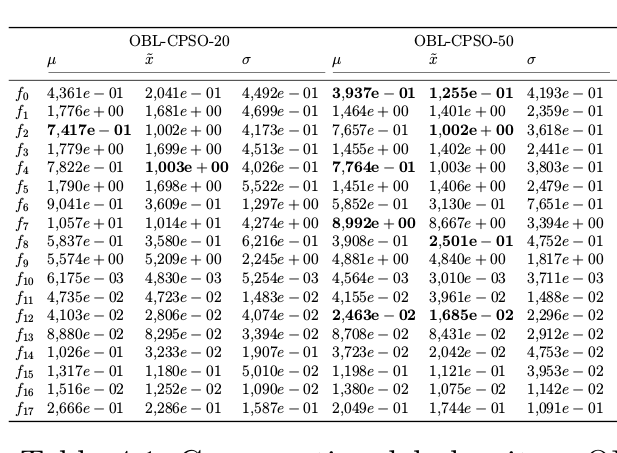
\includegraphics[scale=0.5]{img/oblcpso1}
\end{figure}
\end{frame}

\begin{frame}
\frametitle{Rendimiento de OBL-CPSO}
\begin{figure}
  \centering
	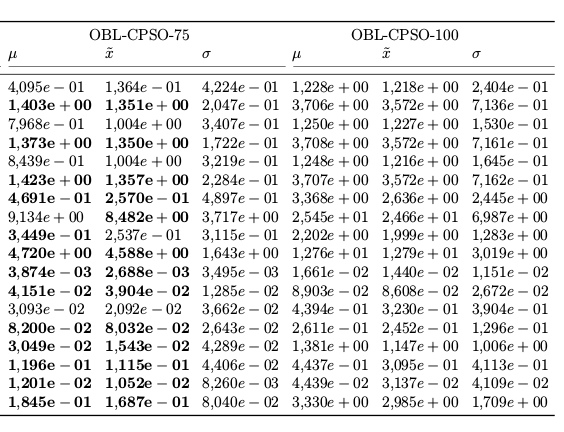
\includegraphics[scale=0.5]{img/oblcpso2}
\end{figure}
\end{frame}

\begin{frame}
\frametitle{Rendimiento de CMA-ES}
\begin{figure}
  \centering
	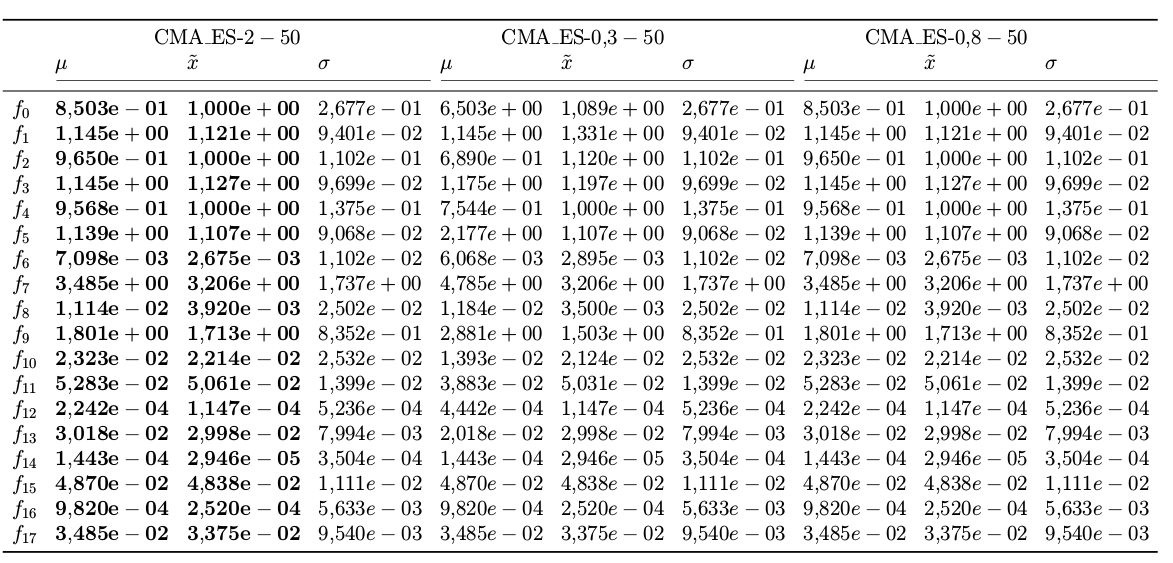
\includegraphics[scale=0.3]{img/cmaF}
\end{figure}
\end{frame}

\begin{frame}
\frametitle{Rendimiento de HSAGS}
\begin{figure}
  \centering
	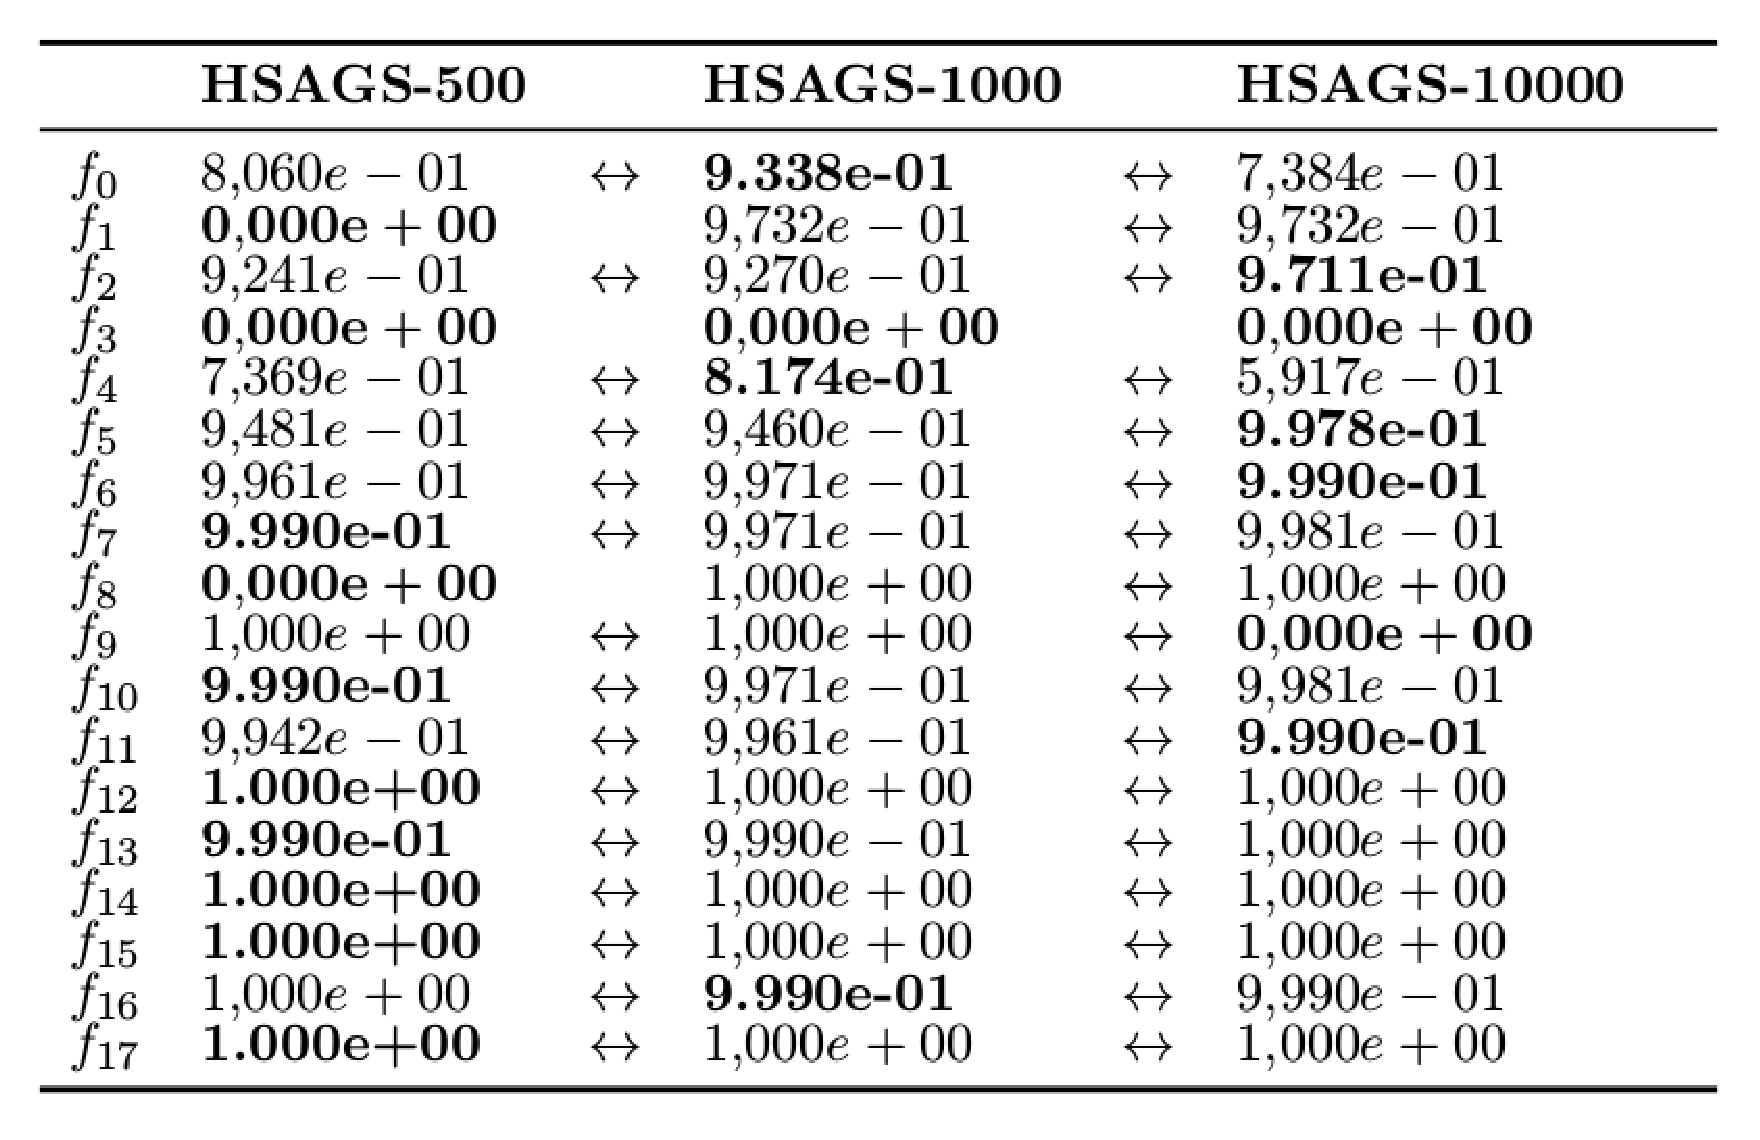
\includegraphics[scale=0.4]{img/hsags}
\end{figure}
\end{frame}

%++++++++++++++++++++++++++++++++++++++++++++++++++++++++++++++++++++++++++++++
\subsection{Comparativa de Rendimiento entre Algoritmos}
\begin{frame}
\frametitle{Comparativa de Rendimiento entre Algoritmos}
\begin{block}{Objetivos del Estudio}
Comparar el rendimiento de cada uno de los algoritmos a la hora de optimizar las funciones propuestas por GenOpt.
\end{block}
\end{frame}

\begin{frame}
\frametitle{Comparativa de Rendimiento entre Algoritmos}
\begin{figure}
  \centering
	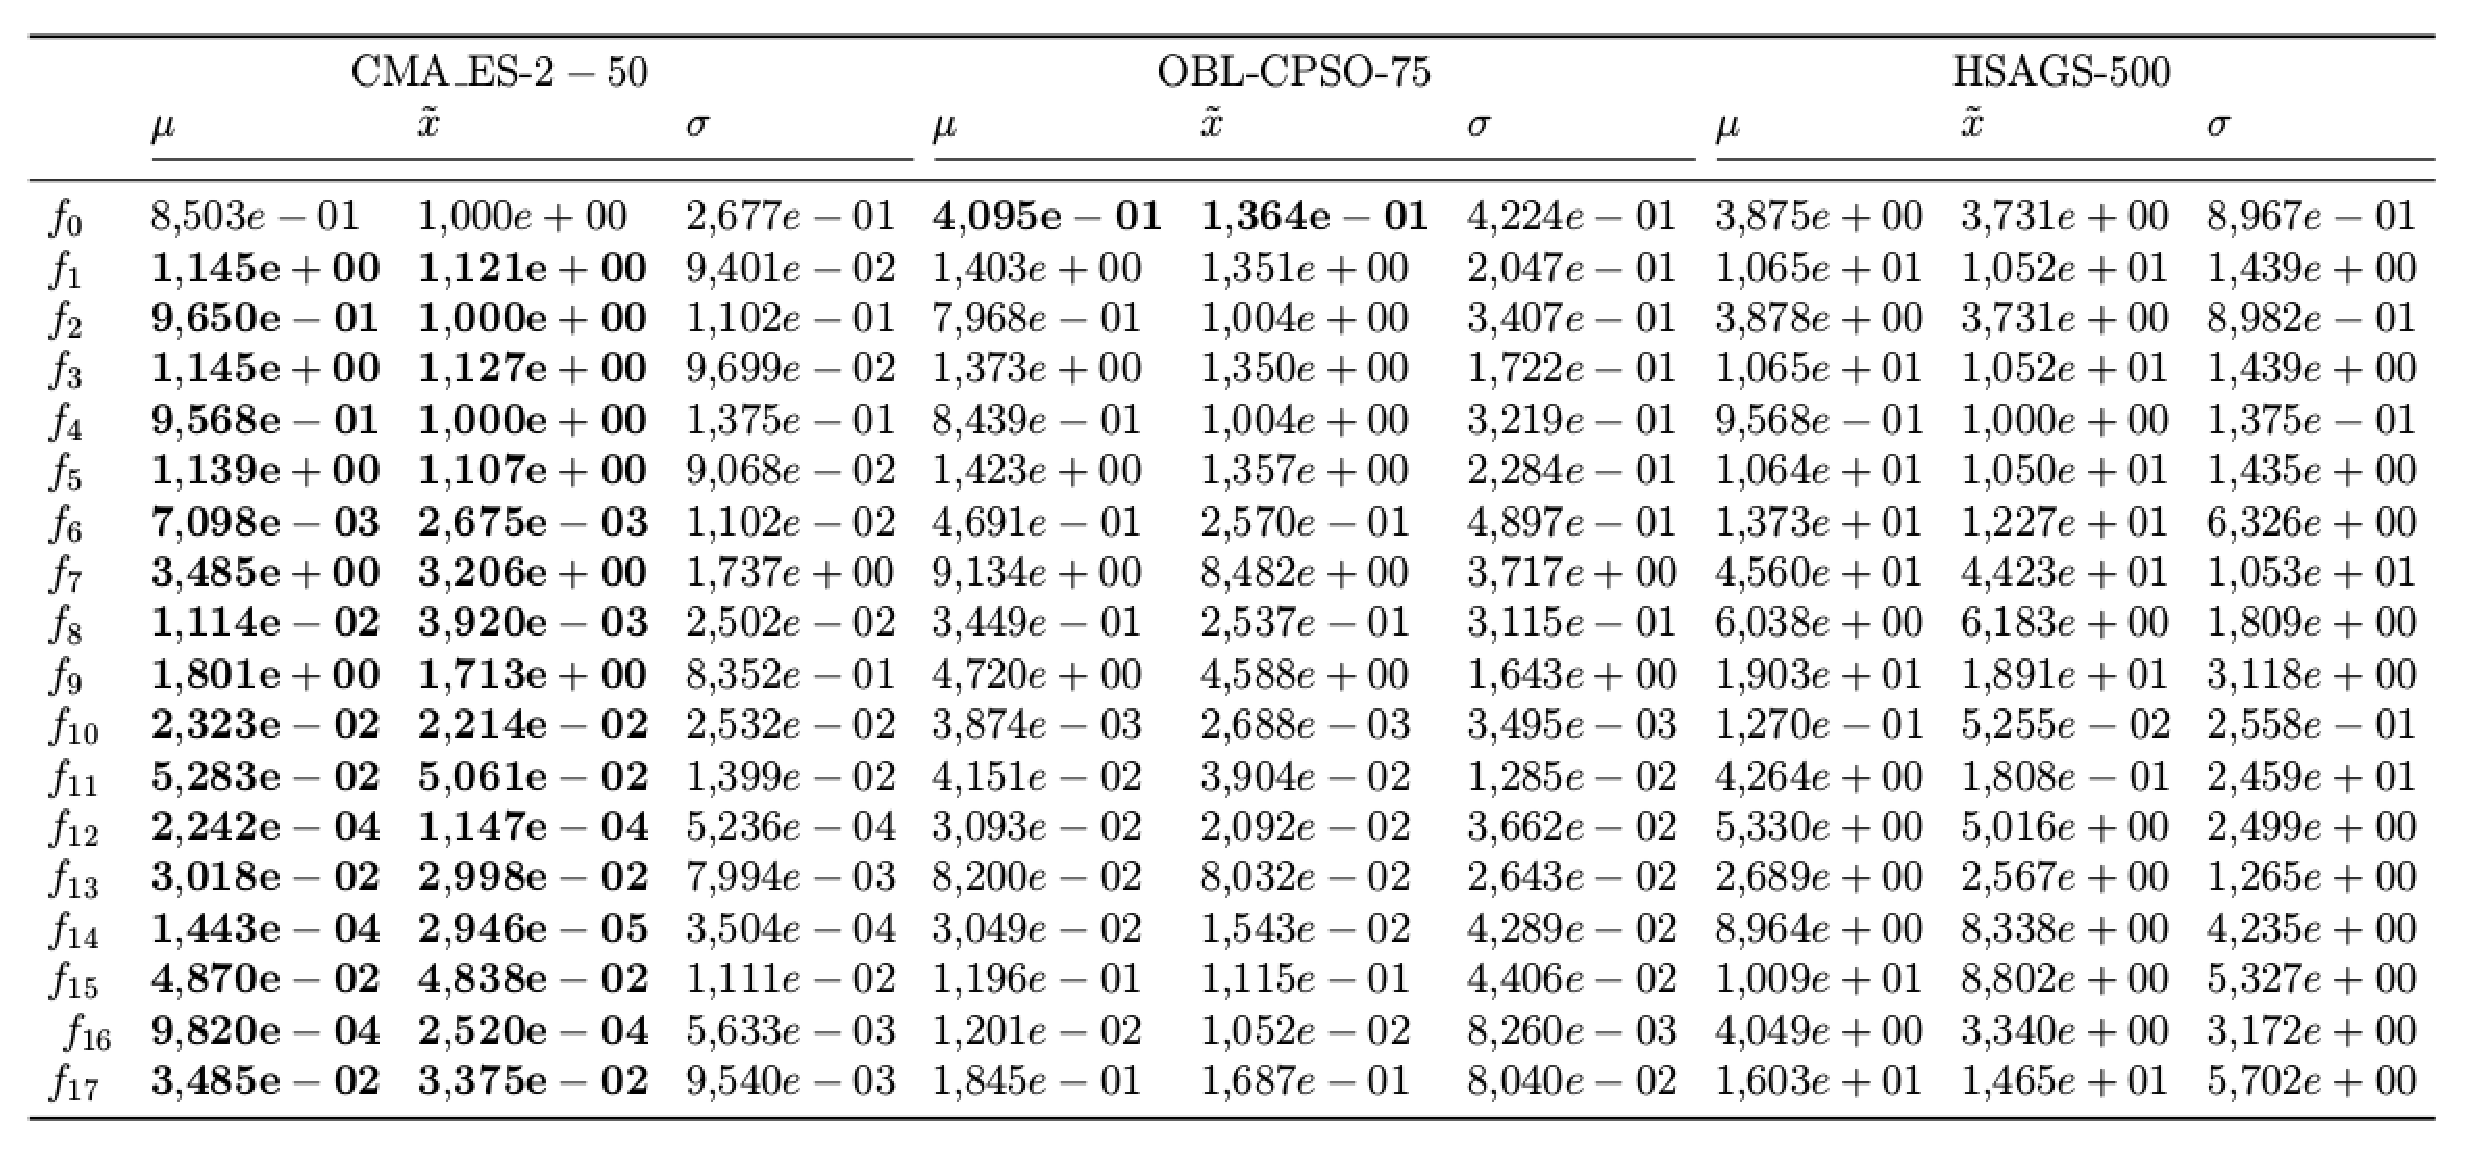
\includegraphics[scale=0.3]{img/finalcmp}
\end{figure}
\end{frame}

%++++++++++++++++++++++++++++++++++++++++++++++++++++++++++++++++++++++++++++++
\subsection{Clasificación en el Concurso GenOpt}
\begin{frame}
\frametitle{Clasificación en el Concurso GenOpt}
\begin{block}{Criterios de Clasificación de GenOpt}
\begin{itemize}
    	  	\item \textbf{High Jump}: mejor valor obtenido en los puntos de control.
    	  	\item \textbf{Target Shooting}: éxito a la hora de alcanzar el óptimo global de la función.
    	  	\item \textbf{Biathlon Score}: media entre el High Jump y Target Shooting.
\end{itemize}
\end{block}
\footnotetext[1]{Manifesto del concurso GenOpt: http://www.genopt.org/genopt.pdf.}
\end{frame}

\begin{frame}
\frametitle{Clasificación en el Concurso GenOpt}
\begin{figure}[!ht]
  \centering
  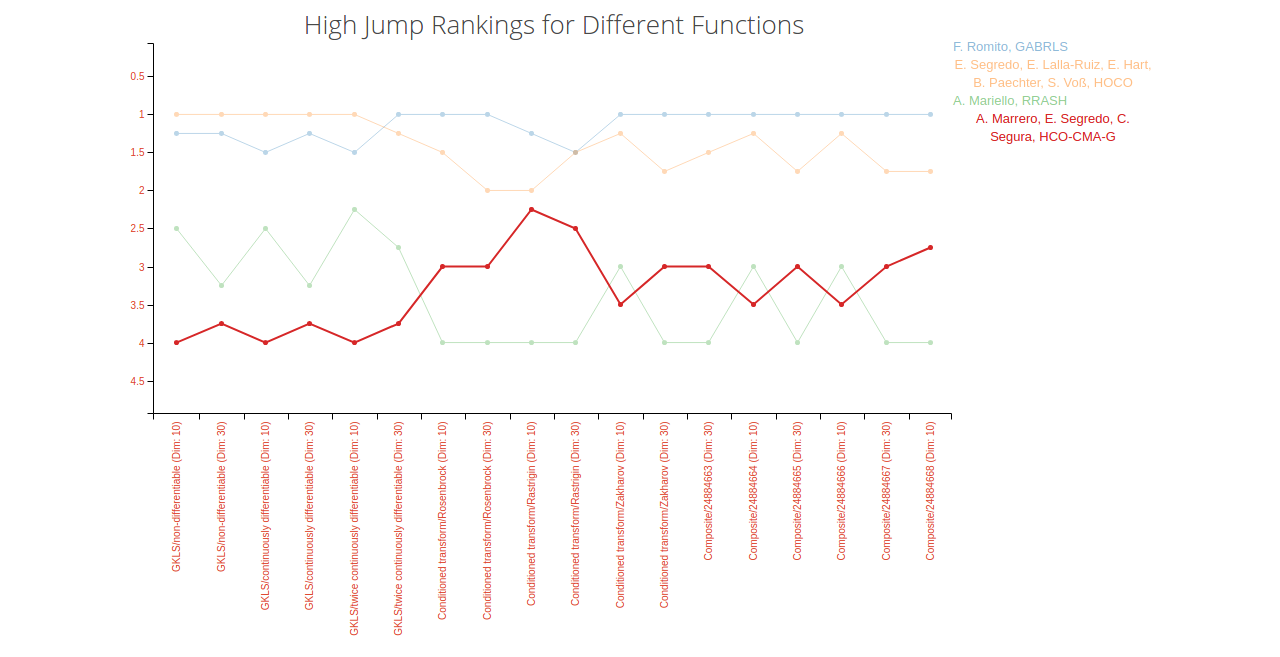
\includegraphics[scale=0.3]{img/highjump}
\end{figure}
\end{frame}

\section{Conclusions and Future Work}
\begin{frame}
\frametitle{Conclusions and Future Work}
\begin{block}{Conclusions}
\begin{itemize}
	\item High amount of parameters increases the complexity to evaluate the performance of the algorithms.
	\item The task of assessing a new modification was really difficult.
	\item CMA-ES algorithm accomplished the \textbf{third place} in the final leaderboard of the GenOpt contest considering the High Jump criterion.
\end{itemize}
\end{block}
\begin{block}{Future Work}
\begin{itemize}
	\item Improve the different tested algorithms.
\end{itemize}
\end{block}
\end{frame}

\section{Bibliografía}
\begin{frame}[allowframebreaks]
        \frametitle{Bibliografía}
        \bibliography{slides}
\end{frame}

 
\begin{frame}
  \centering
  
\includegraphics[width=0.15\textwidth]{img/ullesc.eps}
    \begin{center}
     \Huge{¿Preguntas?} \\
     Gracias por su atención.
    \end{center}
\end{frame}  

%%%%%%%%%%%%%%%%%%%%%%%%%%%%%%%%%%%%%%%%%%%%%%%%%%%%%%%%%%%%%%%%%%%%%%%%%%%%%%%
\title[Desarrollo de Algoritmos Dirigido por Retos]{Desarrollo de Algoritmos Dirigido por Retos}
\author[Alejandro Marrero Díaz]{Alejandro Marrero Díaz}
\institute[ULL]{Universidad de La Laguna}
\date[]{\today}
%++++++++++++++++++++++++++++++++++++++++++++++++++++++++++++++++++++++++++++++  
\begin{frame}
  \centering
  
\includegraphics[width=0.15\textwidth]{img/ullesc.eps}
  \titlepage

  \begin{scriptsize}
    \begin{center}
     Escuela Superior de Ingeniería y Tecnología \\
     Universidad de La Laguna
    \end{center}
  \end{scriptsize}
\end{frame}

\end{document}
